\documentclass[12pt, a4paper]{article}

\usepackage[margin=1in]{geometry}
\usepackage{graphicx}
\usepackage{amsmath}
\usepackage{hyperref}
\usepackage{enumitem}
\usepackage{booktabs}
\usepackage{tikz}
\usetikzlibrary{shapes,arrows.meta,positioning}
\usepackage{fancyhdr}
\usepackage{pdfpages}

% Header/Footer
\pagestyle{fancy}
\fancyhf{}
\fancyhead[L]{\small Internship Report --- Rakuten India}
\fancyhead[R]{\small Ankit Kumar Singh}
\fancyfoot[C]{\thepage}
\renewcommand{\headrulewidth}{0.4pt}

\hypersetup{
    colorlinks=false,
    pdfborder={0 0 0}
}

\begin{document}

% ============================================================
% Title Page
% ============================================================
\begin{titlepage}
    \centering
    \vspace*{2cm}
    
    {\Huge\bfseries Internship Experience Report}
    
    \vspace{0.5cm}
    {\LARGE Data Engineering at Rakuten India}
    
    \vspace{2cm}
    
    {\large \textbf{Submitted by}} \\[8pt]
    {\Large \textbf{Ankit Kumar Singh}} \\[4pt]
    {\large 2021IMT-012} \\[20pt]
    {\large \textbf{Under the supervision of}} \\[8pt]
    {\Large \textbf{Dr. Avadh Kishor}} \\[20pt]
    {\large \textbf{ABV--Indian Institute of Information}} \\
    {\large \textbf{Technology and Management, Gwalior}}
    
    \vfill
    {\large \today}
\end{titlepage}

% Include Offer Letter
\includepdf[pages=-]{offer.pdf}

% ============================================================
% Declaration
% ============================================================
\newpage
\thispagestyle{empty}

\begin{center}
{\Large \bf DECLARATION}
\end{center}
\vspace{0.5cm}
\noindent I hereby certify that the work, which is being presented in the report, entitled \textit{Internship Experience Report --- Data Engineering at Rakuten India}, in fulfillment for the Internship component of the Integrated Post Graduate -- Master of Technology in Information Technology and submitted to the institution is an authentic record of my own work carried out during the period January-2026 to July-2026 under the supervision of Dr. Avadh Kishor. I also cited the reference about the text(s)/figure(s)/table(s) from where they have been taken.

\vspace{1cm}

\begin{center}
	\begin{tabular}{p{0.58\textwidth}p{0.4\textwidth}}
		Dated:  & {\bf{Signature of the candidate}} \\	
	\end{tabular}
\end{center}
\vspace{1.5cm}
\noindent This is to certify that the above statement made by the candidate is correct to the best of my knowledge.

\vspace{1.5cm}

\begin{center}
	\begin{tabular}{p{0.65\textwidth}p{0.4\textwidth}}
		Dated: & {\bf{Signature of supervisor}} \\	
	\end{tabular}
\end{center}

% ============================================================
% Table of Contents
% ============================================================
\tableofcontents
\newpage

% ============================================================
% Chapter 1: Introduction
% ============================================================
\section{Introduction}
\noindent This report summarizes the internship experience at \textbf{Rakuten India}, where the author worked as a \textbf{Data Engineer Intern}. The internship focused on designing and building production-grade data pipelines using modern cloud-native technologies, including Google Cloud Platform (GCP), Apache Airflow, Docker, and BigQuery.

\noindent The report is organized as follows: Section~\ref{sec:about} provides an overview of Rakuten as an organization. Section~\ref{sec:role} describes the role and responsibilities. Section~\ref{sec:projects} details the two major projects undertaken during the internship. Section~\ref{sec:tech} discusses the technical stack used. Section~\ref{sec:learnings} reflects on the key learnings and professional growth.

% ============================================================
% Chapter 2: About Rakuten
% ============================================================
\section{About Rakuten}
\label{sec:about}

\noindent \textbf{Rakuten Group, Inc.} is a Japanese multinational conglomerate headquartered in Tokyo, Japan. Founded in 1997 by Hiroshi Mikitani, Rakuten has grown into one of the world's largest e-commerce and internet companies, operating in over \textbf{30 countries} with more than \textbf{1.6 billion members} across its ecosystem.

\noindent Rakuten's core business segments include:

\begin{itemize}
    \item \textbf{E-Commerce}: Rakuten Ichiba (Japan's largest online marketplace), Rakuten Fashion, and Rakuten Books.
    \item \textbf{Fintech}: Rakuten Card (largest credit card issuer in Japan), Rakuten Bank, Rakuten Securities, and Rakuten Insurance.
    \item \textbf{Mobile \& Telecom}: Rakuten Mobile, offering 4G/5G services as Japan's newest mobile carrier with a cloud-native network architecture.
    \item \textbf{Digital Content}: Rakuten Viber (messaging), Rakuten TV (streaming), and Rakuten Kobo (e-books).
\end{itemize}

\noindent \textbf{Rakuten India}, based in Bangalore, serves as a major engineering hub focusing on platform engineering, data infrastructure, AI/ML research, and product development. The India office contributes to building scalable backend systems and data platforms that power Rakuten's global services.

\begin{table}[h!]
    \centering
    \caption{Rakuten Group --- Key Facts}
    \begin{tabular}{ll}
        \toprule
        \textbf{Attribute} & \textbf{Details} \\
        \midrule
        Founded         & 1997 \\
        Headquarters    & Tokyo, Japan \\
        Founder \& CEO  & Hiroshi Mikitani \\
        Employees       & 30,000+ globally \\
        Revenue         & \$15B+ (FY2024) \\
        Global Presence & 30+ countries \\
        Members         & 1.6+ billion \\
        India Office    & Bangalore (Engineering Hub) \\
        \bottomrule
    \end{tabular}
    \label{table:rakuten_facts}
\end{table}

% ============================================================
% Chapter 3: Role & Responsibilities
% ============================================================
\section{Role and Responsibilities}
\label{sec:role}

\noindent The author joined Rakuten India as a \textbf{Data Engineer Intern} within the Data Platform / Data Engineering team. The role involved designing, building, and maintaining end-to-end data pipelines for structured and semi-structured datasets.

\subsection{Key Responsibilities}

\begin{enumerate}[leftmargin=1.5cm]
    \item \textbf{Pipeline Design \& Development}: Designed and implemented end-to-end ELT/ETL pipelines with proper error handling, logging, and retry mechanisms.
    \item \textbf{Workflow Orchestration}: Built and managed Apache Airflow DAGs for automated scheduling, dependency management, and monitoring of data workflows.
    \item \textbf{Cloud Infrastructure}: Worked extensively with Google Cloud Platform services including Google Cloud Storage (GCS), BigQuery, and Dataproc for cloud-native data processing.
    \item \textbf{Containerization}: Containerized development and orchestration environments using Docker and Colima (Docker Desktop alternative for macOS) to ensure reproducible and portable setups.
    \item \textbf{Data Quality}: Ensured data quality through schema validation, null handling, type enforcement, and data lineage tracking using ETL timestamps and partitioning strategies.
\end{enumerate}

\subsection{Technology Stack}

\noindent The following technologies were used throughout the internship:

\begin{table}[h!]
    \centering
    \caption{Technology stack used during the internship.}
    \begin{tabular}{ll}
        \toprule
        \textbf{Category} & \textbf{Technologies} \\
        \midrule
        Programming Language & Python 3.10+ \\
        Orchestration        & Apache Airflow 2.x \\
        Containerization     & Docker, Colima \\
        Cloud Storage        & Google Cloud Storage (GCS) \\
        Data Warehouse       & Google BigQuery \\
        Distributed Compute  & Google Dataproc (PySpark) \\
        Query Language       & SQL \\
        Version Control      & Git, GitHub \\
        \bottomrule
    \end{tabular}
    \label{table:tech_stack}
\end{table}

% ============================================================
% Chapter 4: Projects
% ============================================================
\section{Projects}
\label{sec:projects}

\noindent During the internship, two major data engineering projects were completed. Both projects followed production-grade engineering practices including modular code design, proper logging, error handling, and documentation.

% --- Project 1 ---
\subsection{Project 1: End-to-End ELT Pipeline (Fintech Dataset)}

\subsubsection{Objective}
\noindent Build a complete \textbf{Extract--Load--Transform (ELT)} pipeline for a fintech dataset, starting from raw data ingestion through data transformation to analytics-ready tables in Google BigQuery.

\subsubsection{Architecture}

\noindent The pipeline follows a four-stage architecture as illustrated in Figure~\ref{fig:elt_pipeline}.

\begin{figure}[h!]
    \centering
    \resizebox{0.9\textwidth}{!}{
    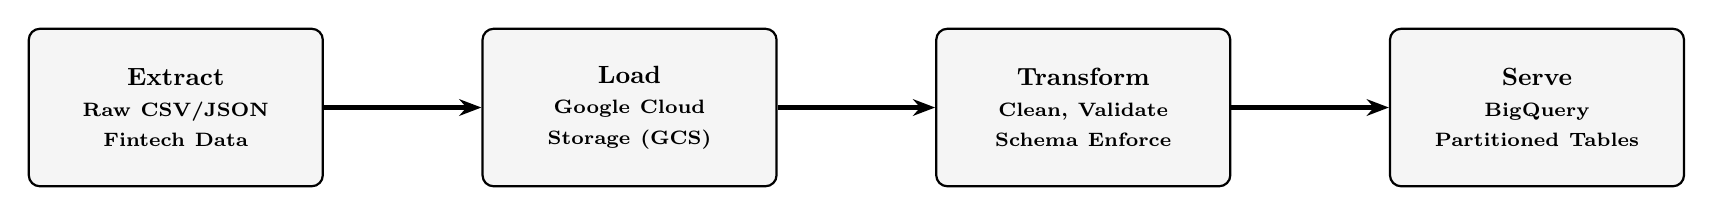
\begin{tikzpicture}[
        node distance=2cm,
        stage/.style={rectangle, draw=black, fill=gray!8, text width=3.5cm, text centered,
                      rounded corners=4pt, minimum height=2cm, font=\small\bfseries,
                      line width=0.8pt},
        arrow/.style={-{Stealth[length=8pt]}, line width=1.5pt}
    ]
        \node[stage] (extract) {\textbf{Extract} \\ {\scriptsize Raw CSV/JSON} \\ {\scriptsize Fintech Data}};
        \node[stage, right=of extract] (load) {\textbf{Load} \\ {\scriptsize Google Cloud} \\ {\scriptsize Storage (GCS)}};
        \node[stage, right=of load] (transform) {\textbf{Transform} \\ {\scriptsize Clean, Validate} \\ {\scriptsize Schema Enforce}};
        \node[stage, right=of transform] (serve) {\textbf{Serve} \\ {\scriptsize BigQuery} \\ {\scriptsize Partitioned Tables}};
        
        \draw[arrow] (extract) -- (load);
        \draw[arrow] (load) -- (transform);
        \draw[arrow] (transform) -- (serve);
    \end{tikzpicture}
    }
    \caption{End-to-end ELT pipeline architecture for the Fintech dataset.}
    \label{fig:elt_pipeline}
\end{figure}

\subsubsection{Implementation Details}

\begin{enumerate}
    \item \textbf{Data Extraction}: Raw fintech data in CSV and JSON formats was ingested from source systems. File naming conventions and folder structures were standardized for organized storage.
    
    \item \textbf{Data Loading to GCS}: Extracted data was uploaded to Google Cloud Storage with proper partitioned folder structures, enabling efficient downstream processing.
    
    \item \textbf{Data Transformation}: The transformation stage included:
    \begin{itemize}
        \item \textbf{Null handling}: Identified and imputed or flagged missing values.
        \item \textbf{Special character cleaning}: Removed or sanitized non-standard characters in text fields.
        \item \textbf{Date/Time transformation}: Standardized date and time formats across all records.
        \item \textbf{Derived columns}: Created \texttt{sales\_yearmonth} column for BigQuery partitioning and \texttt{etl\_timestamp} for data lineage tracking.
    \end{itemize}
    
    \item \textbf{Schema Validation}: Before loading into BigQuery, data was validated against a predefined schema to ensure type consistency, column completeness, and data integrity.
    
    \item \textbf{BigQuery Loading}: Transformed data was loaded into BigQuery tables partitioned by \texttt{sales\_yearmonth}, enabling efficient time-based queries and reduced scan costs.
\end{enumerate}

% --- Project 2 ---
\subsection{Project 2: Fully Automated Pipeline (Car Sales Dataset)}

\subsubsection{Objective}
\noindent Build a \textbf{fully automated, containerized} data pipeline using Docker and Colima on macOS, processing a Car Sales dataset through GCS, Dataproc (PySpark), and BigQuery with \textbf{dynamic cluster management} and zero idle cost.

\subsubsection{Architecture}

\noindent The pipeline follows a five-stage architecture with dynamic infrastructure management, as shown in Figure~\ref{fig:car_pipeline}.

\begin{figure}[h!]
    \centering
    \resizebox{0.95\textwidth}{!}{
    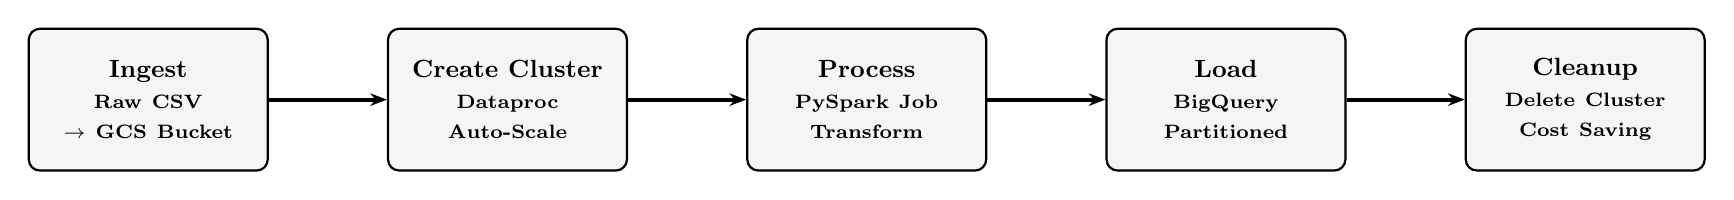
\begin{tikzpicture}[
        node distance=1.5cm,
        stage/.style={rectangle, draw=black, fill=gray!8, text width=2.8cm, text centered,
                      rounded corners=4pt, minimum height=1.8cm, font=\small\bfseries,
                      line width=0.8pt},
        arrow/.style={-{Stealth[length=6pt]}, line width=1.5pt}
    ]
        \node[stage] (ingest) {\textbf{Ingest} \\ {\scriptsize Raw CSV} \\ {\scriptsize $\rightarrow$ GCS Bucket}};
        \node[stage, right=of ingest] (cluster) {\textbf{Create Cluster} \\ {\scriptsize Dataproc} \\ {\scriptsize Auto-Scale}};
        \node[stage, right=of cluster] (process) {\textbf{Process} \\ {\scriptsize PySpark Job} \\ {\scriptsize Transform}};
        \node[stage, right=of process] (load) {\textbf{Load} \\ {\scriptsize BigQuery} \\ {\scriptsize Partitioned}};
        \node[stage, right=of load] (cleanup) {\textbf{Cleanup} \\ {\scriptsize Delete Cluster} \\ {\scriptsize Cost Saving}};
        
        \draw[arrow] (ingest) -- (cluster);
        \draw[arrow] (cluster) -- (process);
        \draw[arrow] (process) -- (load);
        \draw[arrow] (load) -- (cleanup);
    \end{tikzpicture}
    }
    \caption{Fully automated Car Sales pipeline with dynamic Dataproc cluster management.}
    \label{fig:car_pipeline}
\end{figure}

\subsubsection{Implementation Details}

\begin{enumerate}
    \item \textbf{Containerized Environment}: The entire orchestration layer was Dockerized using Docker with Colima as the container runtime on macOS. This provided a lightweight, reproducible alternative to Docker Desktop.
    
    \item \textbf{Data Ingestion}: Raw Car Sales data (CSV format) was uploaded to a GCS bucket with structured folder naming for organized storage.
    
    \item \textbf{Dynamic Dataproc Cluster Creation}: A Dataproc cluster was created on-demand for each pipeline run with the following characteristics:
    \begin{itemize}
        \item \textbf{Auto-scaling}: Worker nodes scaled dynamically based on workload.
        \item \textbf{Zone-aware provisioning}: Clusters were provisioned in zones with available resource quotas.
        \item \textbf{GCP IAM integration}: Service accounts with least-privilege access for secure operations.
    \end{itemize}
    
    \item \textbf{PySpark Processing}: A PySpark job ran on the Dataproc cluster to:
    \begin{itemize}
        \item Clean and preprocess the raw car sales data.
        \item Perform data type transformations and null handling.
        \item Create partitioning columns (\texttt{sales\_yearmonth}) for BigQuery optimization.
        \item Add an \texttt{etl\_timestamp} for data lineage.
    \end{itemize}
    
    \item \textbf{BigQuery Loading}: Processed data was loaded into BigQuery with monthly partitioning and schema validation.
    
    \item \textbf{Cluster Cleanup}: After the PySpark job completed, the Dataproc cluster was automatically deleted, ensuring \textbf{zero idle infrastructure cost}.
    
    \item \textbf{Airflow Orchestration}: The entire workflow was orchestrated via an Apache Airflow DAG with the following task sequence:
    
    \begin{center}
        \texttt{Ingest $\rightarrow$ Create Cluster $\rightarrow$ Submit PySpark $\rightarrow$ Load to BQ $\rightarrow$ Delete Cluster}
    \end{center}
    
    \noindent Each task had configurable retries, timeout handling, and failure notifications.
\end{enumerate}

% ============================================================
% Chapter 5: Technical Comparison
% ============================================================
\section{Technical Comparison of Projects}
\label{sec:tech}

\noindent Table~\ref{table:project_comparison} provides a side-by-side comparison of the two projects.

\begin{table}[h!]
    \centering
    \caption{Comparison of the two internship projects.}
    \begin{tabular}{lll}
        \toprule
        \textbf{Aspect} & \textbf{Project 1 (Fintech)} & \textbf{Project 2 (Car Sales)} \\
        \midrule
        Pipeline Type       & ELT                        & ELT (Automated)             \\
        Language            & Python 3.10+               & Python 3.10+, PySpark       \\
        Orchestration       & Apache Airflow 2.x         & Airflow (Dockerized)        \\
        Container Runtime   & ---                        & Docker + Colima             \\
        Compute             & Local / GCS                & Dataproc (Auto-scale)       \\
        Storage             & Google Cloud Storage        & Google Cloud Storage        \\
        Data Warehouse      & BigQuery                   & BigQuery                    \\
        Cluster Management  & ---                        & Dynamic create/delete       \\
        Partitioning        & Monthly (\texttt{yearmonth}) & Monthly (\texttt{yearmonth}) \\
        Data Validation     & Custom schema checks       & PySpark schema enforcement  \\
        Infrastructure Cost & Minimal                    & Zero idle (ephemeral)       \\
        \bottomrule
    \end{tabular}
    \label{table:project_comparison}
\end{table}

% ============================================================
% Chapter 6: Learnings
% ============================================================
\section{Key Learnings and Takeaways}
\label{sec:learnings}

\subsection{Technical Skills}

\begin{enumerate}
    \item \textbf{Production-Grade Pipeline Design}: Learned to design ELT/ETL pipelines with proper error handling, retry logic, logging, and idempotency --- essential qualities for production systems.
    
    \item \textbf{Containerization}: Gained hands-on experience with Docker and Colima for creating reproducible development environments, ensuring consistency between local development and cloud deployment.
    
    \item \textbf{Cloud-Native Data Processing}: Developed proficiency in GCP services --- GCS for object storage, BigQuery for analytical querying, and Dataproc for distributed PySpark processing.
    
    \item \textbf{Distributed Computing with PySpark}: Wrote PySpark jobs for large-scale data transformation on Dataproc clusters, understanding partitioning, shuffling, and optimization strategies.
    
    \item \textbf{Workflow Orchestration with Airflow}: Designed Airflow DAGs with dependency management, task retries, SLA monitoring, and integration with GCP operators.
\end{enumerate}

\subsection{Professional Growth}

\begin{enumerate}
    \item \textbf{Enterprise Engineering Practices}: Experienced working in a large-scale engineering organization with established coding standards, code review processes, and documentation requirements.
    
    \item \textbf{Cloud Cost Optimization}: Understood the importance of cost-aware infrastructure design --- using ephemeral Dataproc clusters, right-sizing resources, and minimizing idle compute.
    
    \item \textbf{Data Quality as a First-Class Concern}: Learned that data quality (schema validation, null handling, type enforcement) is as critical as pipeline functionality in production environments.
    
    \item \textbf{Collaboration and Version Control}: Worked with Git-based workflows, branch management, pull request reviews, and collaborative documentation practices.
    
    \item \textbf{Fintech Data Governance}: Gained exposure to compliance and governance requirements specific to financial data, including data handling policies and access control mechanisms.
\end{enumerate}

\subsection{Summary}

\noindent The internship at Rakuten India provided a comprehensive, hands-on experience in modern data engineering. By building two end-to-end data pipelines --- one focusing on ELT fundamentals with BigQuery and another on fully automated, containerized infrastructure with Dataproc --- the author gained practical expertise in cloud-native data processing, workflow orchestration, and production-grade pipeline development. These skills are directly applicable to data engineering roles in industry and form a strong foundation for future work in scalable data systems.

\end{document}
